\chapter[Rodovias mais perigosas]{Rodovias mais perigosas}

\begin{enumerate}

\item \textbf{Relatório das rodovias mais perigosas e dos carros mais envolvidos em acidentes}

A BR 262 é uma rodovia transversal brasileira que liga os Estados do Espírito Santo, Minas Gerais, São Paulo e Mato grosso do Sul. Tem início em Vitória (ES) e passa por cidades importantes como Manhuaçu, Belo Horizonte, Araxá, Uberaba, Três Lagoas e Campo Grande. Percorre 999,8 Km no estado de Minas Gerais cortando-o de leste a oeste. Em 2009 apresentou um elevado número de acidentes, foram registrados 9.614 acidentes em que 280 pessoas morreram. Sendo que somente no percurso entre Belo Horizonte e Governador Valadares houveram 2.975 acidentes, no qual 2.159 ficaram feridas e 138 vieram a óbito. Atualmente a rodovia já possui trechos duplicados, mas ainda conta com muitos trechos de mão única.

\begin{figure}[h]
  \centering
  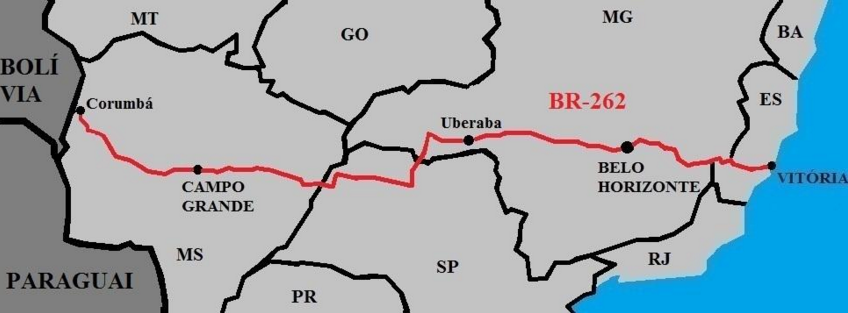
\includegraphics[width=400px, scale=0.5]{figuras/mapa}
  \label{table:mapa}
\end{figure}

\item \textbf{Justificativa}

Em 2014 o Estado de Minas Gerais foi o que apresentou o maior número de acidentes e mortos em rodovias, seguido por Paraná, Santa Catarina, São Paulo e Rio de Janeiro. Essas regiões representam grande parte do contingente populacional do país e, especificamente, o Sudeste responde 49,5\% do PIB do Brasil, sendo São Paulo, Rio de Janeiro e Minas Gerais, respectivamente, os três estados mais ricos do país. Isso faz com que o fluxo rodoviário nessas regiões seja intenso, interferindo no número de acidentes. Seguem alguns dados na tabela abaixo:

\begin{figure}[h]
  \centering
  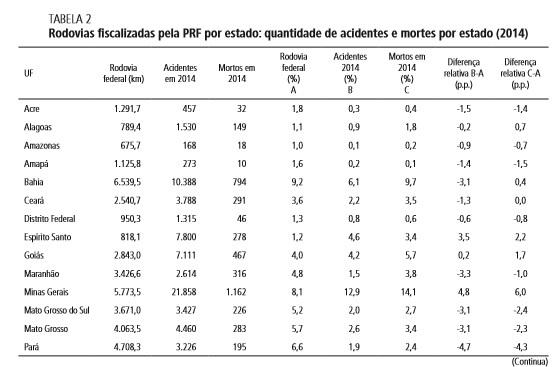
\includegraphics[width=400px, scale=0.5]{figuras/table1}
  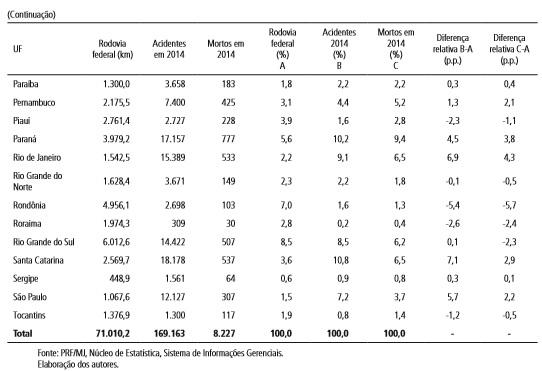
\includegraphics[width=400px, scale=0.5]{figuras/table2}
  \label{table:table}
\end{figure}

Considerando-se os tipos de acidente, verifica-se que a colisão frontal foi responsável por 33,7% das mortes. Nos acidentes desse tipo morreram 40,4 pessoas a cada 100 acidentes. 89,71% das colisões frontais ocorreram em pistas simples, ocasionando 93,91% dos mortos nesse tipo de acidente. A maior causa dos acidentes é a falta de atenção do motorista \cite{ipea2}.

Mesmo não sendo a rodovia mais perigosa e com maior número de acidentes, a BR 262 é considerada uma rodovia perigosa pois apresenta muitos trechos simples de mão dupla, além de algumas deficiências como falta de sinalização e condições ruins de tráfego, o que favorece o implemento do sistema anticolisão veicular. A título de curiosidade, a BR 381( Fernão Dias) é a que mais possui acidentes, porém não são colisões frontais já que inteira duplicada. O trecho entre os Km 490 a 500, na altura de Betim é o que apresenta maior número de acidentes.

\item \textbf{Veículos envolvidos em acidentes}

Em 2013, a PRF registrou um número de 186.474 acidentes nas rodovias federais brasileiras. Em 2014, tínhamos uma frota de 81,3 milhões de veículos.
Os automóveis apresentam o maior percentual de envolvimento nos acidentes de trânsito nas rodovias e também mortes entre todos os modais de transporte, em função do maior número da frota circulante. O gráfico a seguir nos traz números exatos

\begin{figure}[h]
  \centering
  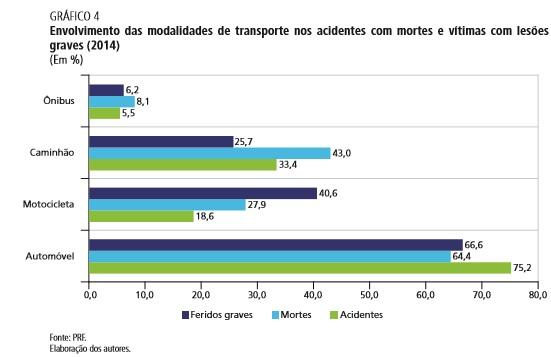
\includegraphics[width=400px, scale=0.5]{figuras/grafico}
  \label{table:mapa}
\end{figure}

Desde 2007 a PRF vem fazendo levantamento de dados sobre quais são os veículos que mais se envolvem em acidentes. Em primeiro lugar temos o Volkswagen Gol, que esteve presente em 14.125 acidentes. Em segundo lugar vem o Fiat Uno, envolvido em 8200 acidentes, seguido pelo Fiat Palio, com registro de 7.041 acidentes. Em quarto lugar vem o Chevrolet Celta, participando de 5.931 acidentes. Em quinto lugar temos a Honda CG 150, envolvida em 5.784 acidentes.
Sendo assim, o sistema anticolisão veicular será implantado no Volkswagen Gol, afim de ilustrar nosso cenário na BR 262 \cite{terra}.

\end{enumerate}
